\subsection{Value of Prediction Accuracy (RQ3)}

Fig.~\ref{fig:alpha} shows RATP as a function of the prediction error level $\alpha$ for the medium-load pooled and fast-track EDs, and Table~\ref{tab:vop} compares, for each of the \NMediumTypes{} medium-load ED types, the best policy that uses predictions with the best policy that does not (FCFS, CTAS or APQ, with CTAS streaming in two-area EDs).

\begin{figure*}[!t]
\centering
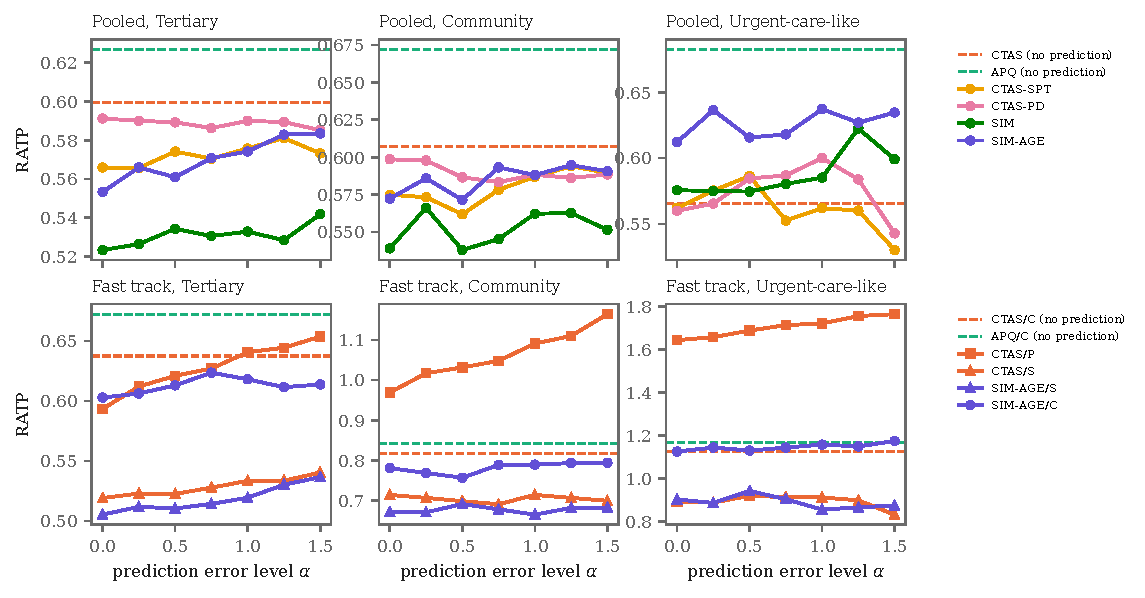
\includegraphics[width=0.9\textwidth]{figures/fig_alpha.pdf}
\caption{RATP against the prediction error level $\alpha$ ($\alpha=0$: perfect information; $\alpha=1$: reference accuracy) for medium-load pooled EDs (top, queue rules) and fast-track EDs (bottom, routing rules). Dashed lines: policies that do not use predictions. \RepsSecondary{} replications per point.}
\label{fig:alpha}
\end{figure*}

\begin{table*}[!t]
\centering
\caption{Gain of the best prediction-based policy over the best policy without predictions (medium load), with perfect information ($\alpha=0$) and reference accuracy ($\alpha=1$), and the largest $\alpha$ tested at which it is still better ($\geq$: better at every $\alpha$ tested).}
\label{tab:vop}
\footnotesize
\setlength{\tabcolsep}{2.5pt}
\begin{adjustbox}{max width=\linewidth}\begin{tabular}{llrrrrrr}
\toprule
 & & \multicolumn{3}{c}{RATP} & \multicolumn{3}{c}{Mean LOS} \\
\cmidrule(lr){3-5}\cmidrule(lr){6-8}
Acuity & Config. & Gain $\alpha{=}0$ (\%) & Gain $\alpha{=}1$ (\%) & Max $\alpha$ & Gain $\alpha{=}0$ (\%) & Gain $\alpha{=}1$ (\%) & Max $\alpha$ \\
\midrule
Tertiary & Pooled & 12.7 & 11.1 & $\geq$1.50 & 1.2 & 1.0 & $\geq$1.50 \\
 & Fast track & 23.3 & 21.5 & $\geq$1.50 & 3.6 & 3.3 & $\geq$1.50 \\
 & Split flow & 12.9 & 11.9 & $\geq$1.50 & 1.1 & 1.1 & $\geq$1.50 \\
Community & Pooled & 11.3 & 7.4 & $\geq$1.50 & 1.8 & 1.6 & $\geq$1.50 \\
 & Fast track & 21.2 & 20.9 & $\geq$1.50 & 0.8 & 0.8 & $\geq$1.50 \\
 & Split flow & 11.5 & 11.5 & $\geq$1.50 & 1.9 & 1.8 & $\geq$1.50 \\
Urgent-care-like & Pooled & 0.9 & 0.6 & 1.50 & 2.6 & 2.5 & $\geq$1.50 \\
 & Fast track & 22.4 & 25.9 & $\geq$1.50 & 2.6 & 5.0 & $\geq$1.50 \\
 & Split flow & 4.1 & 7.0 & 1.50 & 1.7 & 2.0 & $\geq$1.50 \\
\bottomrule
\end{tabular}\end{adjustbox}
\end{table*}

At the reference accuracy the best prediction-based policy had a lower RATP than the best policy without predictions in \VopNBetterAtOneRatp{} of the \NMediumTypes{} ED types and a lower mean LOS in \VopNBetterAtOneLosAllMean. The RATP gain ranged from \VopGainOneMinRatp\% to \VopGainOneMaxRatp\%; it was largest in fast-track EDs and smallest in the pooled urgent-care-like ED, where strict CTAS order is already close to the best. LOS gains were small, at most \VopGainOneMaxLosAllMean\%.

The gains depended little on prediction accuracy. From perfect information to the reference accuracy the RATP gain fell by \VopGainDropRatp{} percentage points on average, and the best prediction-based policy remained better than the best policy without predictions at every error level tested in \VopNAllAlphaRatp{} of the \NMediumTypes{} ED types for RATP and in \VopNAllAlphaLosAllMean{} for mean LOS. At the largest error level ($\alpha=\AlphaMax$) the exact-class accuracy of the service-time prediction is \AccSvcAtMax\%, no better than chance for five classes, and admission is predicted correctly for \AccAdmAtMax\% of patients. That the gains survive such poor predictions indicates that they come mainly from the structure of the rules, not from the information in the predictions. The queue rules remain anchored on the observed CTAS level, and similarity routing sends a larger share of patients to the second area whatever the predictions say (Section~\ref{sec:res:mech}).

Prediction streaming is the exception. It is the one rule in which predictions alone decide where a patient goes, and its RATP rose steadily with $\alpha$ and was worse than CTAS streaming at every error level in the community and urgent-care-like fast-track EDs (Fig.~\ref{fig:alpha}). In the tertiary fast-track ED it beat CTAS streaming when predictions were better than the reference accuracy, but not at the reference accuracy itself. For that rule accuracy matters, and in the other two fast-track EDs even perfect predictions did not make it competitive with the capacity split used here. The answer to how good predictions must be therefore depends on the rule: rules that use predictions to refine an acuity-based order tolerated large errors in our experiments, whereas the rule that streams patients on predictions alone was no better than CTAS streaming at the reference accuracy in any fast-track ED.

\subsection{Sensitivity to Boarding and Diagnostic Intensity}
\label{sec:res:sens}

Table~\aref{tab:sens} reports, for the \NMediumTypes{} medium-load ED types, whether the best policy of the core design remains the best when boarding is longer or diagnostic intensity changes (capacities unchanged), and how much is lost if the core best policy is kept. With light diagnostics the core best policy loses at most \SensLightDiagnosticsRatpRegretMax\% in RATP and \SensLightDiagnosticsLosAllMeanRegretMax\% in mean LOS. With high boarding the best policy for RATP changes in some ED types, but keeping the core best policy costs on average \SensHighBoardingRatpRegret\% in RATP (at most \SensHighBoardingRatpRegretMax\%) and \SensHighBoardingLosAllMeanRegret\% in mean LOS (at most \SensHighBoardingLosAllMeanRegretMax\%); the best queue rules are then \SensHighBoardingBestQueues. Long boarding hits split flow hardest, because admitted patients from the vertical area board in Main beds: in \SensHighBoardingNearSat{} ED types (\SensHighBoardingNearSatList) the median Main-space utilization across policies reached 0.95 or more.

Heavy diagnostics is the most demanding variant. In \SensHeavyDiagnosticsNearSat{} ED types (\SensHeavyDiagnosticsNearSatList) the median Main-space utilization across policies was 0.95 or more (up to \SensHeavyDiagnosticsUtilMax), because capacities were sized for typical diagnostic use. Close to saturation the core best policy lost up to \SensHeavyDiagnosticsLosAllMeanRegretMax\% in mean LOS; elsewhere it held up, which suggests that the results are least reliable for an ED operating close to the capacity of its Main area.


